\clearpage
\section{Datumsfunktionen}

\subsection{Allgemeines}

Für Excel beginnt die Zeitrechnung am 0.1.1900. Das klingt seltsam, hat aber seinen Ursprung in  einer längst vergessenen Software, nämlich dem Tabellenkalkulationsprogramm Lotus 123.
Dieses Programm hatte einen Bug, denn es sah das Jahr 1900 als Schaltjahr an, was aber nicht stimmt. Um mit dem damaligen Platzhirsch kompatibel zu sein, baute Microsoft absichtlich
diesen Fehler ein. Deswegen beginnt die Microsoftsche Zeitrechnung mit dem 0.1. und nicht mit dem 1.1., damit ab dem 1. März 1900 der Kalender wieder stimmt.

Für Excel ist jedes Datum eine Zahl, beginnend mit dem 0.1.1900 mit der Zahl 0. Der 1.1.1900 ist dann 1 und so weiter. Der 1.1.1950 ergibt demnach 18264 und der 11.11.2009 den Wert 40128. Sobald Sie nun eine Zelle als Datum formatieren, weiß Excel, dass es diese Zahl
in ein Datumsformat wandeln soll.
	\begin{figure}[H]
		\centering
			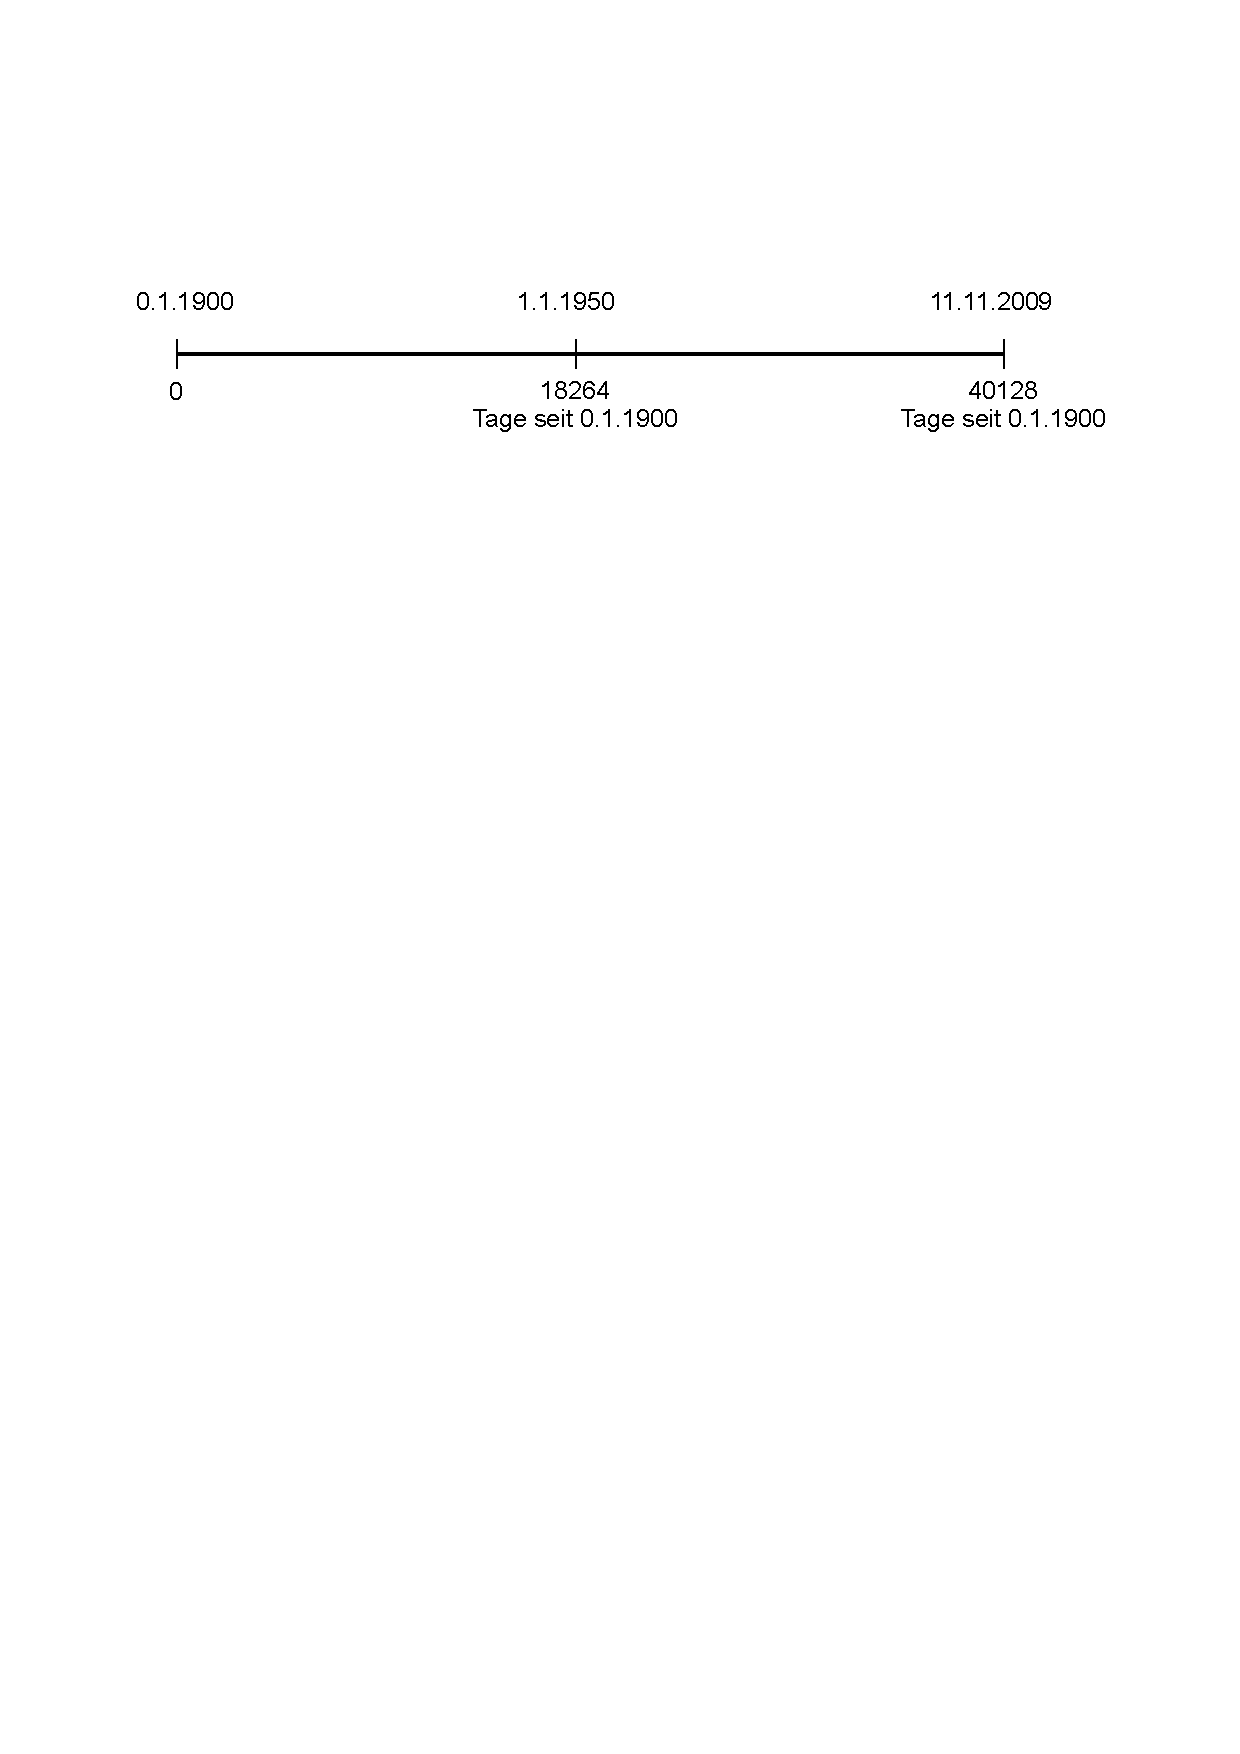
\includegraphics{_OpenOffice/datum.pdf}
		\caption{Datumsdarstelung in Excel}
		\label{fig:datum}
	\end{figure}

%\placefigure[middle,force][fig:datum]{}{\externalfigure[datum]}

Der Vorteil dieser Darstellung ist, dass man mit Daten einfach rechnen kann.
%\placefigure[middle,force][fig:datumdiff]{}{\externalfigure[datumdiff]}
	\begin{figure}[H]
		\centering
		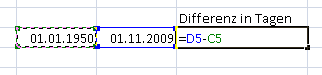
\includegraphics{images/datumdiff.png}
		\caption{Rechnen mit Datumsangaben}
		\label{fig:datumdiff}
	\end{figure}


Der Haken ist nur der, dass Excel in seiner grenzenlosen Intelligenz das Format der Quellzelle übernimmt, welche ein Datum ist. Dadurch erhalten sie nicht die Differenz in Tagen, sondern ein seltsames Datum.
%\placefigure[middle,force][fig:datumdiff2]{}{\externalfigure[datumdiff2]}
	\begin{figure}[H]
		\centering
		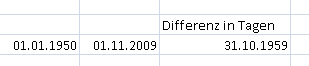
\includegraphics{images/datumdiff2.png}
		\caption{Formatfehler der Datumsberechnung}
		\label{fig:datumdiff2}
	\end{figure}




Sie müssen nun die Zelle auf das Format Standard oder Zahl ändern um das richtige Ergebnis anzuzeigen.
%\placefigure[middle,force][fig:datumdiff3]{}{\externalfigure[datumdiff3]}
	\begin{figure}[H]
		\centering
		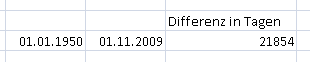
\includegraphics{images/datumdiff3.png}
		\caption{Tagesdifferenz als Zahl formatiert}
		\label{fig:datumdiff3}
	\end{figure}



%\placefigure[right,force][fig:alter1]{}{\externalfigure[alter1]}
	\begin{figure}[H]
		\centering
		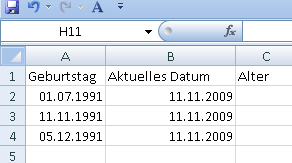
\includegraphics{images/alter1.png}
		\caption{Altersdifferenzen, Ausgangslage}
		\label{fig:alter1}

	\end{figure}


Berechnen wir nun als Beispiel das Alter von drei Freunden, welche alle im selben Jahr geboren wurden und zwar am 1.7.1991, am 11.11.1991 und am 5.12.1991. Der Zeitpunkt der Berechnung ist am Geburtstag des zweiten, also am
11.11.1991. Wir wissen, dass Excel ein Datum intern als Zahl behandelt. Dadurch kann man ein Datum vom anderen abziehen.

Erstellen wir nun die Berechnungformel Schritt für Schritt für den ältesten der drei Freunde, welcher am 1.7.1991 geboren wurde.
%\placefigure[middle,force][fig:datum2]{}{\externalfigure[datum2]}
	\begin{figure}[H]
		\centering
		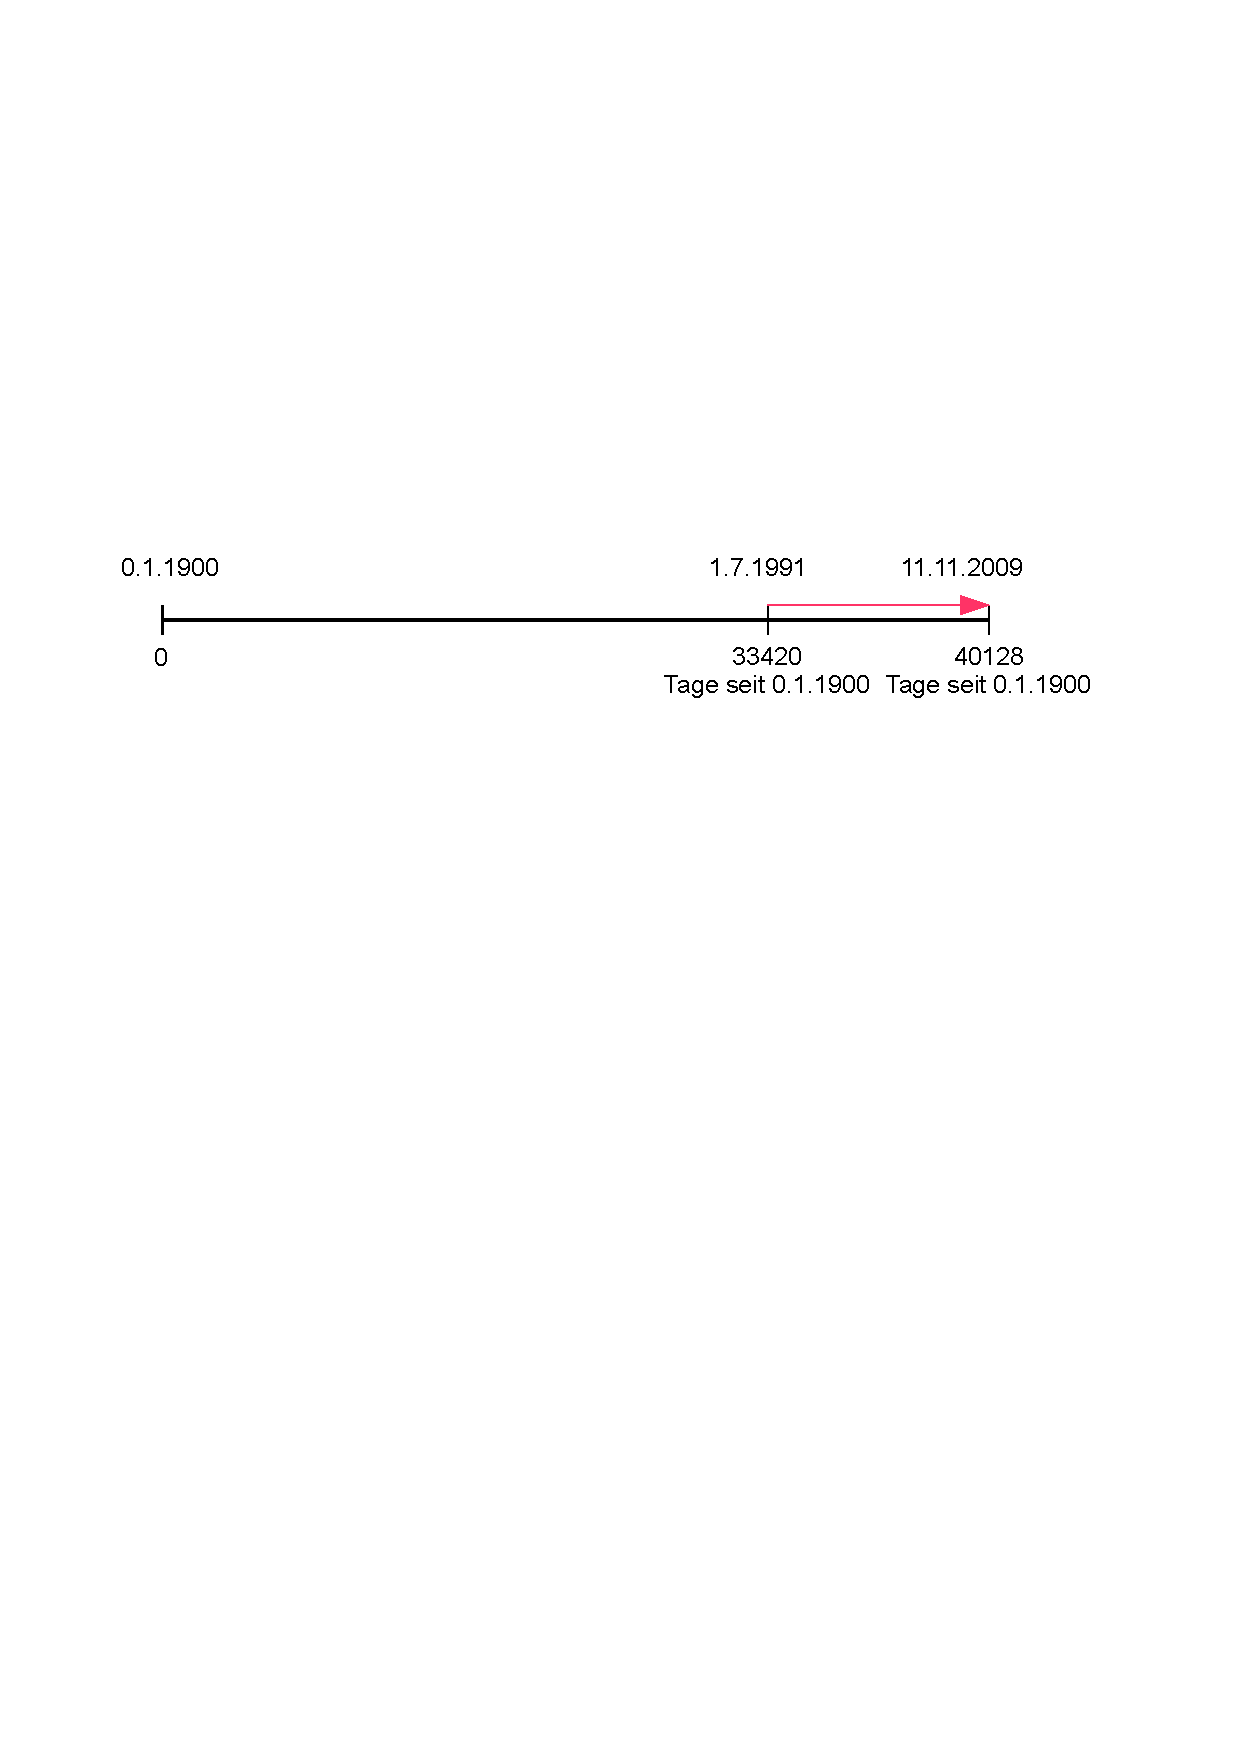
\includegraphics{_OpenOffice/datum2.pdf}
		\caption{Altersdifferenz auf der Zeitachse}
		\label{fig:datum2}

	\end{figure}


Aus der \figref{fig:datum2} kann man erkennen, dass zwischen dem 11.11.2009 und dem 1.7.1991 genau 40128-33420 Tage liegen, was 6708 Tagen entspricht. Tragen wir nun einmal diese einfache Formel ein und sehen uns das Ergebnis an.
%\placefigure[middle,force][fig:alter2]{}{\externalfigure[alter2]}
	\begin{figure}[H]
		\centering
		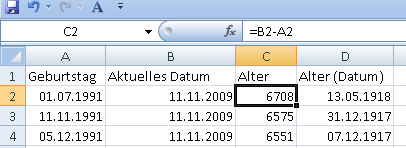
\includegraphics{images/alter2.png}
		\caption{Berechnete Altersdifferenzen}
		\label{fig:alter2}
	\end{figure}


In Zelle \xlc{C2} steht die Formel \stmt{=B29-A2}. In der Spalte \xlc{C9} ist das Alter in Tagen als Zahl formatiert zu sehen. In der Spalte \xlc{D} dagegen ist der Inhalt der Spalte \xlc{C} als Datum formatiert zu sehen. Es ist erkennbar, dass das Jahr 1917, beziehungsweise
1918, etwas mit dem Alter zu tun haben muss. In der unteren Abbildung ist die Erklärung dafür. Nehem Sie die Differenz der beiden Zeitpunkte und betrachten Sie diese vom Anbeginn der Microsoftschen Zeitrechnung aus.
%\placefigure[middle,force][fig:datum3]{}{\externalfigure[datum3]}
	\begin{figure}[H]
		\centering
		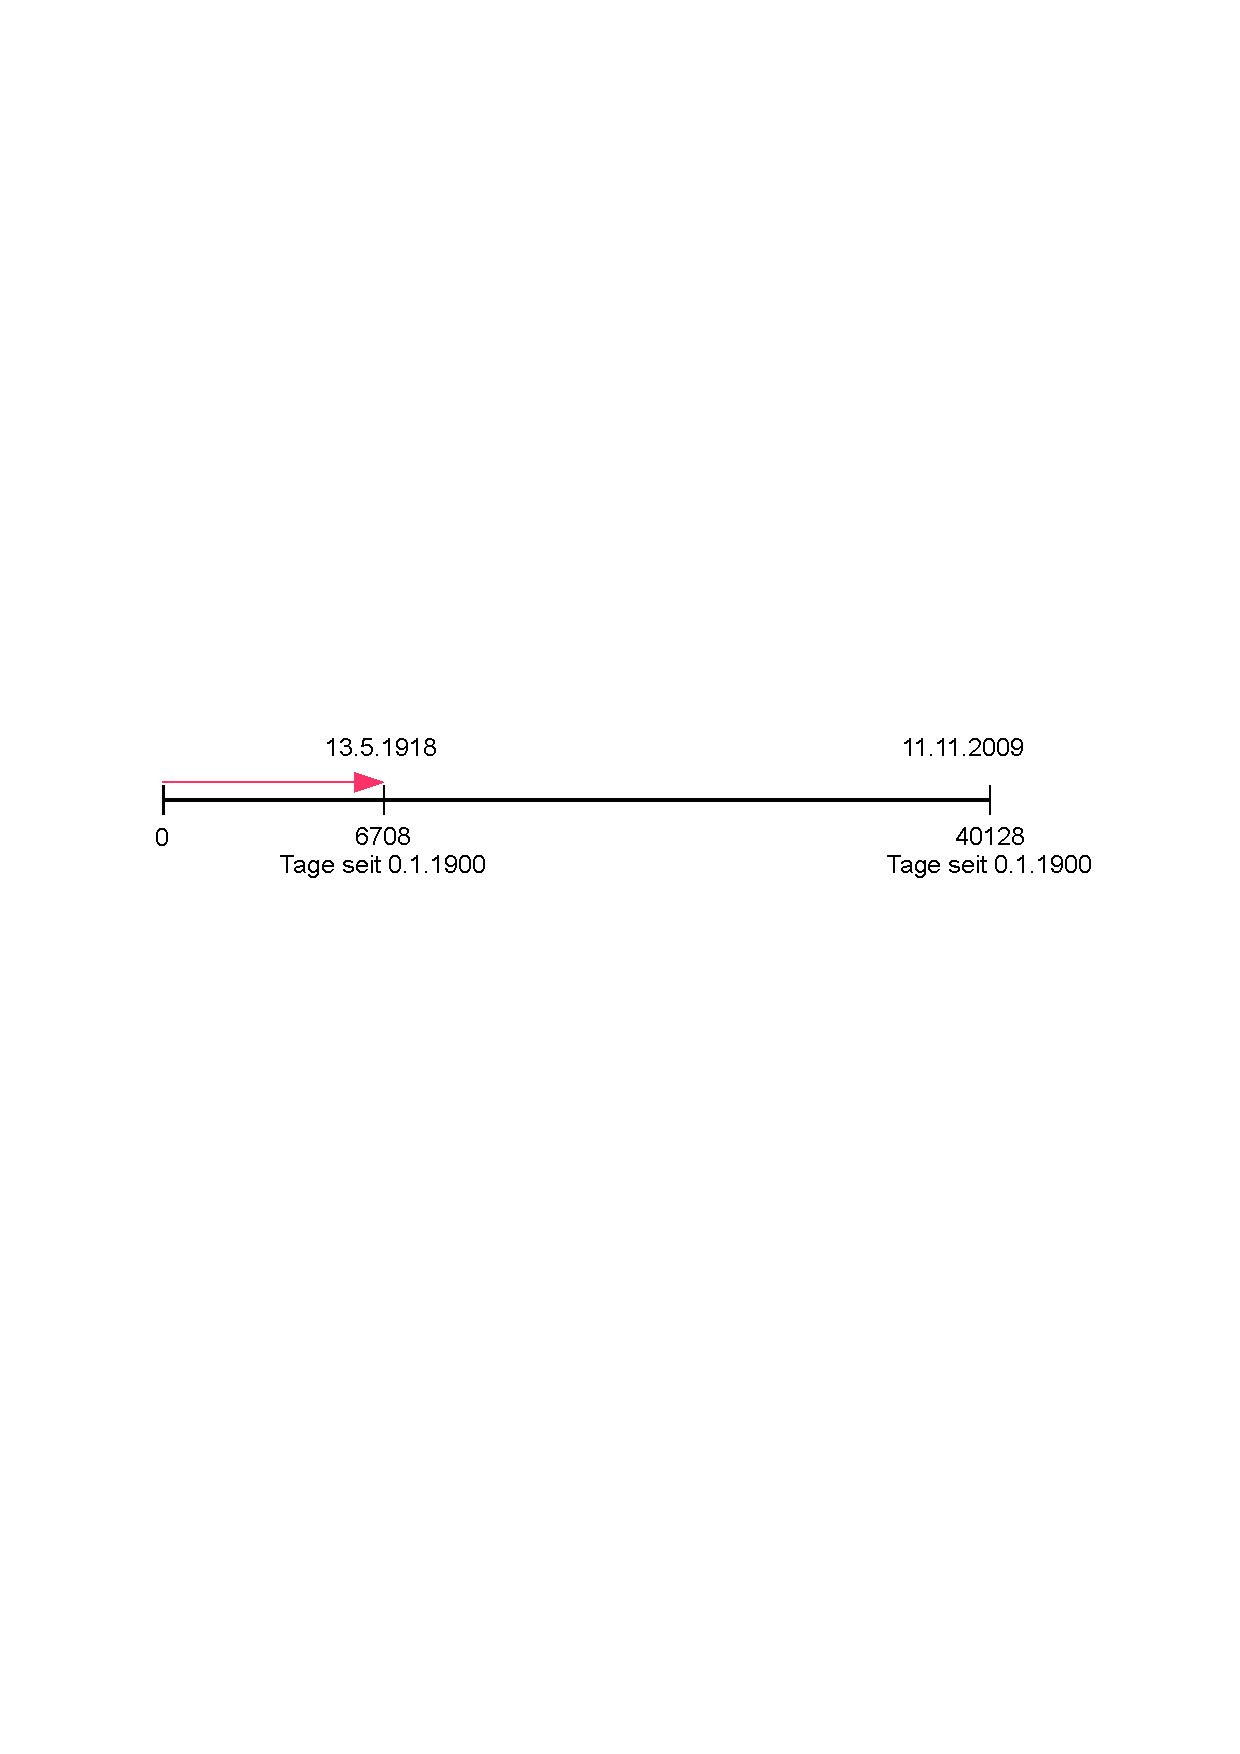
\includegraphics{_OpenOffice/datum3.pdf}
		\caption{Differenzalter auf der Zeitachse}
		\label{fig:datum3}
	\end{figure}



Um das eigentliche Alter in Jahre zu erhalten sind jetzt noch 2 Schritte notwendig
\begin{itemize}
	\smallitemize
	\item Mittels der Funktion \stmt{JAHR()} aus dem Differenzdatum nur die Jahreszahl extrahieren.\\
	Mit \stmt{=JAHR(B2-A2)} erhalten Sie 1917, beziehungsweise 1918
	\item Den Beginn der Microsoftschen Zeitrechnung, also 1900, abziehen
	Mit \stmt{=JAHR(B2-A2)-1900} erhalten Sie 17, beziehungsweise 18
\end{itemize}

Damit scheint das Ergebnis erreicht zu sein. Leider nur scheinbar, denn am Tag des Geburtstages wird ein falsches Alter angezeigt. Um das zu korrigieren, addiert man einfach einen Tag zur Differenz zwischen beiden Daten. Das Ergebnis sieht dann wie folgt aus.
%\placefigure[middle,force][fig:alter3]{}{\externalfigure[alter3]}
	\begin{figure}[H]
		\centering
		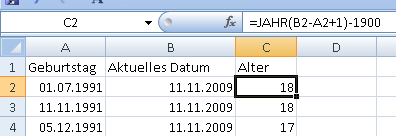
\includegraphics{images/alter3.png}
		\caption{Tatsächliche Altersdifferenz}
		\label{fig:alter4}
	\end{figure}

\subsection{Übersicht}

\begin{description}[labelindent=0cm, leftmargin=7cm, font=\mdseries, labelwidth=5cm,style=nextline]
	
	\item[\stmt{HEUTE()}] Liefert das aktuelle Datum\\
		Z.B.  \stmt{HEUTE()} $\Rightarrow$ 01.09.2015
	\item[\stmt{JETZT() }] Liefert das aktuelle Datum samt Uhrzeit\\ 
		Z.B. \stmt{JETZT} $\Rightarrow$ 21.02.2014 12:00:23
\item[\stmt{TAG(\syntax{Datum})}] Liefert den Tag eines Datums als Ganzzahl\\
		Z.B. \stmt{TAG(\upquote{21.02.2014})} $\Rightarrow$ 21
\item[\stmt{MONAT(\syntax{Datum})}] Liefert das Monat eines Datums als Ganzzahl\\
		Z.B. \stmt{MONAT("21.02.2014")} $\Rightarrow$ 2
\item[\stmt{JAHR(\syntax{Datum})}] Liefert das Jahr eines Datums als Ganzzahl\\
		Z.B: \stmt{JAHR("21.02.2014")} $\Rightarrow$ 2014
\item[\stmt{DATUM(\syntax{Jahr}; \syntax{Monat}; \syntax{Tag})}] Erstellt aus 3 Ganzzahlen ein Datum\\
	Z.B. Datum(21; 2; 2014) $\Rightarrow$ 41691\\
	Diese Funktion ist eine der wichtigsten Datumsfunktionen, weil Sie eine beliebige Addition oder Subtraktion von Jahren, Monaten und Tagen ermöglicht und daraus ein neues Datum erstellen kann.
\item[\stmt{MONATSENDE(\syntax{Datum}, \syntax{Monat})}] Liefert das Monatsende als Datum (Zahl) zurück, das eine bestimmte Anzahl von Monaten vor bzw. nach einem Datum liegt.\\
	Z.B. \stmt{("21.02.2014"; 3)} $\Rightarrow$ 31.05.2014
\item[\stmt{WOCHENTAG(\syntax{Datum}; \syntax{Typ})}] Liefert den Wochentag eines Datums als Ganzzahl zurück, wobei die Typangabe (Default = 1) entscheidet, welcher Wochentag mit welcher Zahl beginnt. (bei Default gilt 1=So, 2=Mo,3=Di,..)\\
Z.B. (z.B. \stmt{("21.02.2014"; 1)} $\Rightarrow$ 6
\item[\stmt{TEXT(\syntax{Datum};"\syntax{Format}") }] Gibt ein Datum entsprechend dem ausgewählten Format an\footnote{\url{https://support.office.com/de-at/article/TEXT-Funktion-20d5ac4d-7b94-49fd-bb38-93d29371225c?ui=de-DE&rs=de-AT&ad=AT}}.\\
	Z.B.  \stmt{TEXT("21.02.2014"; "TTT")} $\Rightarrow$ Fr
\item[\stmt{DATEDIF(\syntax{Startdatum}; \syntax{Enddatum}; \syntax{Einheit})}] Liefert die Differenz als Ganzzahl zwischen zwei Datumswerten. Als Einheit kann man "Y", "M" oder "D" angeben. Es ist zu beachten, dass das Startdatum immer vor dem Enddatum liegen muss.\\
Z.B. \stmt{DATEDIF(HEUTE(); "24.12.2014"; "D")} $\Rightarrow$ 306
\item[\stmt{ARBEITSTAG(\syntax{Startdatum};\syntax{Tage}; \syntax{Freitage}) }] Liefert das Datum des nächsten (oder zurückliegenden) Arbeitstages durch Addition oder Subtraktion von Tagen zu einem Startdatum unter Berücksichtigung eventueller Freitage (Matrix).
\item[\stmt{NETTOARBEITSTAGE(\syntax{Beginndatum}; \syntax{Enddatum}; \syntax{Freitage}) }] Liefert die Anzahl der Arbeitstage zwischen einem Anfangsdatum  und einem Enddatum unter Berücksichtigung eventueller Freitage (Matrix).
\item[\stmt{EDATUM(\syntax{Ausgangsdatum} ;\syntax{Monate})}] Liefert das Datum (Zahl) zurück, das eine bestimmte Anzahl von Monaten vor bzw. nach einem Ausgangsdatum liegt.\\
Z.B. \stmt{EDATUM("29.02.2016"; -12)} $\Rightarrow$ 28.02.2015
\item[\stmt{KALENDERWOCHE(\syntax{Datum}; \syntax{Typ}) }] Liefert die Kalenderwoche eines Datums als Ganzzahl zurück.\\
Typ 1: Woche mit dem 1.1. ist die 1. Kalenderwoche (amerikanisches System)\\
Typ 21: Woche, die den 1. Donnerstag im Jahr hat, ist die Kalenderwoche 1 oder die den 4.1. beinhaltet (entspricht ISO EU-Standard).
\end{description}



\subsection{Zusammenfassung}
\begin{itemize}
	\item In Excel werden Datumswerte als Ganzzahl interpretiert. Das Standard-Datumsystem basiert darauf, dass der 1.1.1900 der Zahl 1 entspricht. Das letzte interpretierbare Datum ist der 31.12.9999, was der Zahl 2.958.465 entspricht.
	\item Auf Grund des Jahrtausendwechsels sind Jahreszahlen im vierstelligen Format anzugeben. Die zweistelligen Jahreszahlen 00-29 werden als 2000 bis 2029 interpretiert, 30 bis 99 hingegen als 1930 bis 1999.

	\item Da In Excel Datums- und Uhrzeitangaben als Zahlen repäsentiert werden, kann man daher auch mittels mathemathischer Operatoren, wie Addition und Subtraktion, mit Datumswerten rechnen.	
	
\end{itemize}